\chapter{Curriculum Vitae}

\section{Personal Details}

\begin{tabular}{@{}lp{12cm}@{}}
\toprule
%\textbf{ECSE 429 Questions} & \textbf{F18} \\ 
%\toprule
%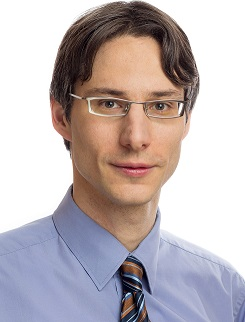
\includegraphics[width=.2\textwidth]{figures/VarroD-2015-small.jpg} &  \\ \midrule
Full name:  & Dániel Varró \\ %\midrule
Contact address: &  3480 Rue University, McConnell Engineering Building \newline
Department of Electrical and Computer Engineering \newline
McGill University \newline
Montreal, QC, Canada, H3A 0E9\\ %\midrule
Phone: &  +1-514-3983681 \\ %\midrule
Email: &  \href{mailto:daniel.varro@mcgill.ca}{daniel.varro@mcgill.ca} \\ %\midrule
\bottomrule
\end{tabular}

\section{Education and Degrees}

\begin{yearlist}
\item[2013] Doctor of Science (DSc); Hungarian Academy of Sciences  
\item[2011] Habilitation; Budapest University of Technology and Economics (in short: BME) 
\item[2004] PhD in Software Engineering (official name: Technical Informatics); BME
\item[2000] MSc in Software Engineering (official name: Technical Informatics); BME 
\end{yearlist}

%\newline This degree is a formal prerequisite of full professorship in Hungary. \\


\section{Academic and Professional Experience}
\subsection{Academic Positions}
\begin{yearlist}
\item[2016-] Professor, Electrical and Computer Engineering (ECE) Department, McGill University
\item[2015- 2020] Research Chair of MTA-BME Lendulet Cyber-Physical Systems Research Group; \\ Hungarian Academy of Sciences 
\item[2014-] Professor, Dept. of Measurement and Inf. Systems, BME  (on unpaid leave since 08/2016)
\item[2014] Visiting Professor, Dept. of Computer Science, McGill University, Canada
\item[2014] Visiting Professor, D\'epartemente d'informatique et de recherche op\'ertionnelle (DIRO), Universit\'e de Montr\'eal, Canada
\item[2009-2014] Associate Professor (tenured), Dept. of Measurement and Inf. Systems, BME 	
\item[2005-2009] Assistant Professor, Dept. of Measurement and Information Systems, BME 
\item[2003-2005] Lecturer, Dept. of Measurement and Information Systems, BME
\end{yearlist}

\subsection{Research Visits} 
\begin{yearlist}
\item[2014] Universit\'e de Montr\'eal (Prof. Houari Sahraoui) and McGill University (Prof. Hans Vangheluwe),  6 months
\item[2005] TU Berlin, Germany (1 month, with Prof. Hartmut Ehrig, SEGRAVIS Grant)
\item[2004] TU Berlin, Germany (1 month, with Prof. Hartmut Ehrig, SEGRAVIS Grant)
\item[2003] Univ. Paderborn, Germany (3 months, with Prof. Gregor Engels, SEGRAVIS) 
\item[2001] SRI International, US (4 months, with Dr. John Rushby) 
\end{yearlist}

\subsection{Industrial Positions and Entrepreneurship} 
\begin{yearlist}
\item[2013-] Co-founder of IncQuery Labs Ltd. (Co-founder and Strategic advisor) 
\item[2006-2014] Co-founder and Vice-President of Research and Development at OptXware Ltd. 
\end{yearlist}

\subsection{Membership in Professional Societies and Committees}
\begin{yearlist}
\item[2018-] \textbf{Member}: The McGill Sustainability Systems Initiative (MSSI)
\item[2016-] \textbf{Member}: McGill Institute for Aerospace Engineering (MIAE)
\item[2011-] 3 times \textbf{Elected member}: Informatics Committee of Hungarian Academy of Sciences (a total of 15 senior members are elected in the field of in computer science and software engineering)
\item[2009-2015] \textbf{Vice president}: John von Neumann Computer Society 
\item[2006-] \textbf{Member}: IEEE Computer Society 
\end{yearlist}


\section{Awards and Honors} 

Six major awards since affiliated to McGill University. 
\begin{yearlist}
\item[2018] \textbf{Distinguished Reviewer Award} (at ICSE 2018: 40th (IEEE/ACM) International Conference on Software Engineering: 11 out of 101 program committee members)
\item[2018] \textbf{Best Tool Paper Award} (at MODELS 2018: ACM/IEEE 21st Int. Conference on Model Driven Engineering Languages and Systems: 1 out of 10 tool papers)
\item[2018] \textbf{EASST Best Paper Award} (at ETAPS 2018: European Joint Conferences on Theory and Practice of Software: selected 1 out of over 140 papers)
\item[2017] \textbf{Csanád Imreh Award} (by OTDT Hungary): \newline I was the first ever awardee of the prize (awarded in the field of software engineering and computer science for Hungarian researchers below the age of 41) commemorating the Hungarian computer scientist who tragically died in 2017 at the age of 41.  
\item[2016] ACM \textbf{Distinguished Paper Award} (at MODELS 2016: 19th IEEE/ACM International Conference on Model Driven Engineering Languages and Systems) 
\item[2016] IEEE \textbf{10-Year Most Influential Paper Award} \newline (at VL/HCC 2016: IEEE Symposium on Visual Languages \& Human-Centric Computing for a paper presented at VL/HCC 2005 conference) 
%\hrule
\item[2014] Springer \textbf{10-Year Most Influential Paper Award} \newline (at MODELS 2014: 17th IEEE/ACM International Conference on Model Driven Engineering Languages and Systems for a paper presented at UML2004 conference) 
\item[2014] \textbf{Best Paper Award} (at IEEE CSMR-WCRE 2014 Software Evolution Week) 
\item[2014] \textbf{STEM Award} by Tempus Foundation for innovative education methods (introducing Apache VCL cloud based labs)
\item[2013] Springer \textbf{Best Paper Award} (MODELS 2013: 16th IEEE/ACM International Conference on Model Driven Engineering Languages and Systems: 1 out of 47 accepted papers) 
\item[2011] ACM \textbf{Distinguished Paper Award} (ASE 2011: 26th IEEE/ACM International Conference on Automated Software Engineering) 
\item[2010-2013] \textbf{J\'anos Bolyai Scholarship} (Design and Analysis Techniques for the Certification of Model Transformations): A national award of the Hungarian Academy of Sciences for young scholars. It can be awarded
at most twice in lifetime.
\item[2009] \textbf{Distinguished Tutor}: Bi-annual award for the supervisionof MSc students carrying out early research with 3 awardees in Computer Science biannually. It requires 10 years of successful tutoring (I became the youngest ever awardee). 
\item[2009] Springer \textbf{Best Paper Award} and ACM \textbf{Distinguished Paper Award} (MODELS
2009: The 12th IEEE/ACM International Conference on Model Driven Engineering Languages and Systems: 1 out of 58 papers) 
\item[2005-2008] \textbf{J\'anos Bolyai Scholarship} (Design and Analysis Techniques for Automated Model Transformations) 
\item[2003] \textbf{J\'anos Kem\'eny Prize } (An annual award in Hungary for young scholars below the age of 35 issued by the John von Neumann Computer Society)
\end{yearlist}

\section{Invited talks}

A career total of 37 invited talks, 9 invited talks since joining McGill University. 

\begin{yearlist}
\item[2018] Design space exploration for graph model generation  (Search Based Model Engineering Workshop at King's College London) 
\item[2017] \textbf{Keynote talk}: Automated Graph Model Generation for Smart and Safe Cyber-Physical Systems (Consortium for Software Engineering Research CSER 2017)
\item[2017] Incremental Queries and Reactive Transformations (DSM-TP 2017 Int. Summer School)
\item[2017] Formal Verification and Validation in Domain-Specific Languages (DSM-TP 2017 Summer School)
\item[2016] Graph-based  Design and Analysis Tools for Smart and Safe Cyber-Physical Systems (NASA Jet Propulsion Lab) 
\item[2016] Model-based Tools for Engineering Cyber-Physical Systems (McGill University Professor Talks)
\item[2016] Scalable  Graph-based techniques for smart cyber-physical systems (Papyrus Industrial Consortium)
\item[2016] Incremental Model Queries and Transformations (DSM-TP 2016 International Summer School) 
\item[2016] Models and Queries for Smart and Safe Cyber-Physical Systems (CSCS 2016 Conference, Szeged)
\item[2016] Challenges for Smart and Trustworthy Cyber-Physical Systems (Ericsson University Day 2016 Budapest)
\item[2016] \textbf{Keynote talk}: Incremental Queries and Transformations: From Concepts to Industrial Applications  (SOFSEM 2016: 42nd Int. Conf. on Current Trends in Theory and Practice of Computer Science) 
\item[2015] EMF/Ecore-based DSL engineering (at Dagstuhl \#15062:  Domain-Specific Languages)
\item[2015] EMF-IncQuery: Incremental Evaluation of Model Queries (DSM-TP 2015 Int. Summer School)  
\item[2015] VIATRA: Advanced Tools by Reactive Transformations (DSM-TP 2015 Int. Summer School) 
\item[2014] \textbf{Plenary Talk}: Generic and Meta-Transformations (Most Influential Paper Presentation at @MODELS 2014, Valencia, Spain)
\item[2014] Incremental Model Queries over the Cloud (SERENE 2014 Int. Autumn School, Hungary)
\item[2014] EMF-IncQuery: Incremental Evaluation of Model Queries (DSM-TP 2014 Int. Summer School)
\item[2014] Incremental Model Queries for Model Driven Software Engineering (DSM-TP 2014 Int. Summer School)
\item[2014] Distributed Incremental Model Queries (at Ericsson Modeling Day, Sweden)
\item[2014] \textbf{Keynote talk}: Distributed Incremental  Model Queries over the Cloud: Engineering and Deployment Challenges (CloudMDE 2014 Workshop @MODELS 2014)
\item[2014] Distributed Incremental Model Queries (at ISIS, Vanderbilt University, US)
\item[2014] \textbf{Keynote talk}: Distributed Incremental Model Queries (GT-VMT 2014 Workshop @ETAPS 2014) 
\item[2013] Validation of Complex Domain-Specific Modeling Languages (at Dagstuhl Seminar 13211 Automatic Reasoning on Conceptual Schemas)
\item[2013] \textbf{Keynote talk}: V\&V Challenges for Models, Queries and Transformations in Design Tools for Avionics (VOLT 2013 Workshop)
\item[2013] Model queries for secure collaborative modeling (EternalS 2013 Workshop) 
\item[2012] \textbf{Keynote talk} at 16th European Conference on Software Maintenance and Reengineering (CSMR 2012, Szeged, Hungary) 
\item[2012] Developing Design Tools for Critical Embedded Systems: A Model Transformation Playground
(at RISC, Hagenberg, Austria) 
\item[2010] Designing Domain-Specific Languages (at University of Szeged, Hungary)
\item[2009] Model driven development of configuration tables (at Rockwell Collins, US)
\item[2009] Model transformation development (at SENSUS International Summer School, Hungary)
\item[2009] Service deployment by model transformation (at SENSUS Summer School, Hungary)
\item[2008] Precise model transformations for tool integration (at TU Berlin, Germany)
\item[2007] Model transformation by example (at ISIS, Vanderbilt University, US)
\item[2007] Model-Driven Deployment of Services to Standards Compliant Reliable Middleware (at Dagstuhl Seminar 07061 Autonomous and Adaptive Web Services)
\item[2007] The VIATRA2 model transformation framework (at TU Darmstadt, Germany)
\item[2004] Towards Automated Formal Verification of Visual Modeling Languages
(at Dagstuhl Seminar 04101 Language Engineering for Model-Driven Software Development) 
\item[2003] Model checking visual modeling languages (at SRI International, US) 
\end{yearlist}

\newpage 

\section{Projects and Funding} 
%\lhead{Third party funding} 


\subsection{Canadian Projects (as PI or co-PI)}
\textbf{Total acquired own funding}: approx. 600,000 CAD 

\begin{yearlist}
\item[2019 - 2020] \textbf{NSERC-Engage}: SmartTarget: Automated identification of performance regressions in a multi-tier web applications; NSERC Engage project proposal (with Predikat Inc). Under review, PI, own funding: 25,000 CAD 
\item[2018-2023] \textbf{NSERC-CRD}: Digital Multidisciplinary Analysis and Design Optimization Platform for Aeroderivative Gas Turbines, NSERC Collaborative Research and Development Grant, PI: M. Kokkolaras (McGill), co-PIs: H. Moustapha (ETS), 
D. Varr\'o:  Total/own funding: 1,177,500 CAD / 294,375 CAD (25\%)
\item[2016 - 2021] \textbf{NSERC-DG}: Model-based Design and Validation Techniques for
Smart and Safe Cyber-Physical Systems (RGPIN-2016-04573), NSERC Discovery Grant, PI, own funding: 230,000 CAD 
\item[2017] \textbf{NSERC-SDG}: LiveIDE: Live Integrated Development Environment for Software-Intensive Communication Systems, PI: D. Varr\'o, co-PIs: G. Mussbacher, J. Kienzle (McGill), H. Sahraoui, E. Syriani (UdeM): Submitted as a Strategic Partnership Grant, recommended for funding by NSERC as a Collaborative Research and Development Grant with Ericsson. The CRD contract was not signed as the Ericsson project lead left the company: Total funding: 571,275 CAD
\item[2016-2019] \textbf{McGill Startup Fund}: Initial research support: 55,000 CAD 
\item[2016-2019] \textbf{McGill EUSF}: 4 teaching support funds by EUSF: total around 7,500 CAD 
\end{yearlist}


\subsection{Collaborative European Projects (as Site Leader or Research Coordinator at BME)}

\begin{yearlist}
\item[2013-2016] \textbf{MONDO}: Scalable Modelling and Model Management on the Cloud (EU-FP7-ICT-STREP, own funding: 420,000 EUR) 
\item[2010-2013] \textbf{E-Freight}: European e-Freight Capabilities for Co-modal Transport (EU-FP7-SST-IP, own funding: 260,000 EUR) 
\item[2009-2012] \textbf{SecureChange}: Security Engineering for Lifelong Evolvable Systems (EU-FP7-FET-IP, 231101-2009, own funding: 250,000 EUR) 
\item[2006-2010] \textbf{DIANA}: Distributed, equipment Independent environment for Advanced avioNic Applications (EU-STREP, FP6-2005-Aero-1, own funding: 410,000 EUR) 
\item[2005-2010] \textbf{SENSORIA}: Software Engineering for Service Oriented
Overlay Computers (FP6 European IP, IST-016004, own funding: 300,000 EUR)  
\end{yearlist}


\subsection{Hungarian National Projects (as PI)}

\begin{yearlist}
\item[2015-2020] \textbf{MTA-BME Lend\"ulet} Cyber-Physical Systems Research Group, 520 000 EUR
\item[2010-2014] \textbf{CERTIMOT}: Design and Analysis Techniques for Certifiable Model Transformations (ERC-HU-09: Starting Grant, 370 000 EUR: My ERC Starting Grant proposal went to the final round at EC with a score of 7/8;
%and it was recommended for funding but became out of budget, 
finally it was partially funded by the Hungarian Research Agency.
\end{yearlist}



\subsection{Industrial Research Grants and Projects at BME} 

\begin{yearlist}
\item[2012-2014] Collaborative project with \textbf{Embraer} on model-driven avionic design tools (Acronym: TRANS-IMA, funding: 200 000 EUR) 
\item[2013-14] Collaborative project with \textbf{Ericsson} on modeling and verification of statecharts (funding: 20 000 USD)
\item[2006-2010] Two collaborative projects with \textbf{Nokia Research Centre}
on high-availability service platforms, and on model-driven development techniques (funding: 40 000 EUR)
\item[2007] \textbf{IBM Faculty Award}: A framework for the model-driven design and analysis of standards-compliant IT infrastructure management (by IBM TJ Watson Research Centre, funding: 20,000 USD)  
\item[2006] \textbf{IBM Faculty Award}: Model based deployment of services to standards-compliant reliable IBM middleware (by IBM TJ Watson, funding: 10,000 USD) 
\item[2005] \textbf{IBM Faculty Award}: Model Transformation Engineering as a complement to IBM Process Modeling Technologies (by IBM TJ Watson, funding: 6,000 USD)  
\end{yearlist}



%\textbf{Total own funding}: approx. 2.2 million EUR \\
\textbf{Total acquired own funding} (before joining McGill): approx. 2.5 million EUR. \\
%\textbf{Total acquired own funding}: approx. 4.65 million CAD\\
(This excludes funding I secured as a co-founder of IncQuery Labs Ltd, which also exceeds 800K EUR, but not reported in the current CV.)
%(This excludes funding I secured as a co-founder of IncQuery Labs Ltd, which exceeds 1.2 million CAD, but not report due to non-disclosure agreements.)

%\subsection{Further Project Participation} 


\subsection{Participation in Collaborative Research Projects (as Contributor)}
\begin{yearlist}
\item[2009-2011] \textbf{INDEXYS}: INDustrial EXploitation of the genesYS cross-domain architecture (ARTEMIS-2008-1-100021) 
\item[2006-2008] \textbf{RESIST}: Resilience for Survivability in IST (EU-FP6 Network of Excellence)  
\item[2004-2007] \textbf{DECOS}: Dependable Embedded Components and Systems (FP6 European IP) 
\item[2002-2006] \textbf{SEGRAVIS}: Syntactic and Semantic Integration of
Visual Modelling Techniques (Research Training Network) 
\end{yearlist}

%\textbf{NECSIS}: \years{2014} (An Automotive Partnership Canada project)  \\

\subsection{Participation in National Research and Innovation Projects (as  Contributor)}
\begin{yearlist}
\item[2005-2007] An MDA based product family for service dependability and optimization (GVOP-2005-3.3.1, in Hungarian)  
\item[2005-2006] EC-Conforming Certification of Safety Equipments for Hungarian Railways (GVOP-2004-3.1.1) 
\item[2001-2003] Operation Research Methods for the Analysis and Verification of IT Systems (OTKA T038027) 
\item[2000-2002] Framework for the Development and Testing of Dependable, Safety-Critical Systems (IKTA-00065/2000) 
\item[2000-2001] Formal Methods in Informatics (MEH 96/2000) 
\item[1999-2001] Automated Verification and Validation of UML Models for IT Systems (OTKA T030804) 
\end{yearlist}

%\cvsubsection{National Projects on innovative exploitation of academic results (as Major Contributor)}


\subsection{Major Open Source Software Projects}
Two of the following projects were founded after joining McGill University.

\begin{yearlist}
\item[2016-] VIATRA Generator (Co-Founder): Open source project for automated generation of graph models \newline \url{https://github.com/viatra/VIATRA-Generator} 

\item[2004-] VIATRA Model Transformation Framework (Founder): Official open source project hosted by the Eclipse Foundation \newline \url{http://www.eclipse.org/viatra} 

\item[2010-2016] EMF-IncQuery: Incremental queries over EMF models (Co-founder) 
%\url{http://www.eclipse.org/incquery/} \\

\item[2014-] MASSIF: Matlab Simulink Integration Framework for Eclipse (Co-founder) \newline 
\url{https://github.com/viatra/massif} 

\item[2017-] Gamma Statechart Composition Framework (Contributor): An open source project with a high-level composition language with precise semantics and model checking backends. \newline \url{http://gamma.inf.mit.bme.hu/} 

\end{yearlist}

\newpage 

\section{Significant University Duties}
%\lhead{Teaching and University Duties} 

\subsection{Departmental Committees (at McGill)}

\begin{yearlist}
\item[2018-] \textbf{Program director}, Software engineering co-op program 
\item[2018-2019] \textbf{Member}, Undergraduate Advising Committee
\item[2018-2019] \textbf{Member}, Curriculum Committee 
\item[2018] \textbf{Member of Qualifying Exam Committee}: M\'arton B\'ur
\item[2017-2019] \textbf{Member}, Departmental Search Curriculum 
\item[2017-2018] \textbf{Member}, Promotions and Reappointment Committee 
\item[2017] \textbf{Member of Qualifying Exam Committee}: Anastasios Alexandridis
\item[2016-2018] \textbf{Member}, Chairman's Advisory Commitee 
\item[2016-2018] \textbf{Member}, Departmental Tenure Commitee 
\item[2016-2017] \textbf{Member}, Graduate Student Financing Committee
\end{yearlist}

\subsection{Faculty-level and University-level Committees (at McGill)}
\begin{yearlist}
\item[2017-2020] \textbf{Representative of Engineering Faculty}, Council of Graduate and Postdoctoral Studies (CGPS) 
\item[2018-] \textbf{Member}, Committee on Student Exchange and Study Abroad 
\item[2018] \textbf{Pro-Dean}, Art History \& Communication Studies, McGill University 
\item[2017-] \textbf{Member}, GitHub Enterprise evaluation committee 
\end{yearlist}

\subsection{Major Academic Duties in Hungary}

\begin{yearlist}
\item[2014-] \textbf{Core member}: Informatics Doctoral School, BME   
\item[2014-2016] \textbf{External member}: Informatics Doctoral School, University of Szeged  
\item[2014-2016] \textbf{Specialization coordinator}:  Systems Engineering Specialization (undergrad), BME   
\item[2012-2016] \textbf{Operative lead}: Fault Tolerant Systems Research Group, BME   
\item[2012-2016] \textbf{Member}: Operative Committee, Dept. of Measurement and Inf. Systems, BME  
\end{yearlist}

\section{Graduate Supervision and Tutoring}
%\cvsubsection{PhD students (main supervisor)}

\subsection{Summary of supervision record}

%An overview of my record as a supervisor of graduate and (McGill) undergraduate students is provided in \autoref{tab:graduate-supervisor-overview}.

\begin{table}[htb]
\footnotesize
\begin{tabular}{@{}p{3cm}lp{2.5cm}p{2.7cm}p{3.5cm}@{}}
\toprule
\textbf{Category} & \textbf{Supervision} & \textbf{Total supervised (defended)} & \textbf{McGill supervised (defended)} & \textbf{Details} \\
\midrule
PhD & main & 11 (7) & 5 (3) & see \autoref{tab:phd-supervised}  \\
PhD & co- & 8 (4) & 4 (1) & see \autoref{tab:phd-cosupervised} \\
MEng/MSc thesis & main/co & 28 (23) & 5 (0) & see \autoref{tab:msc-supervised} \\
Undergrad (DP) & main & -- & 29 & 9 projects, see \autoref{tab:ug-supervised} \\ %(ECSE 456/457)
Undergrad (SURE\footnote{Summer Undergraduate Research in Engineering})  & main & -- & 9 & 6 projects, see \autoref{tab:ug-supervised} \\
\bottomrule
\end{tabular}
%\caption{Overview of graduate supervision data}
%\label{tab:graduate-supervisor-overview}
\end{table}

%\textbf{PhD students (main supervisor)}: 11 supervised (7 defended), see \autoref{tab:phd-supervised} \\
%\textbf{PhD students (co-supervisor)}: 8 students (4 defended), see \autoref{tab:phd-cosupervised} \\
%\textbf{MEng/MSc thesis students}: 28 (co-)supervised (23 defended), see \autoref{tab:msc-supervised} \\
%\textbf{Undergraduate students (at McGill)}: 35 students, 9 Design projects (ECSE 456/457), 6 SURE (Summer Undergraduate Research in Engineering) projects, see \autoref{tab:ug-supervised} \\

\subsection{International Awards Won by PhD students}

4 major international prizes (3 since joining McGill) 
\begin{yearlist}
\item[2018] \emph{G. Sz\'arnyas}: ACM Student Research Competition (SRC): 2nd place at SIGMOD 2018 (main scientific forum in database research),
\item[2017] \emph{C. Debreceni}: ACM SRC: 1st Prize at IEEE/ACM MODELS 2017 conference (main scientific forum of my research area)
\item[2016] \emph{G. Sz\'arnyas}: ACM SRC: 1st Prize at MODELS 2016; 
\item[2014] \emph{G. Sz\'arnyas}: Best Presentation Award at STAF 2014 Doctoral Symposium
\end{yearlist}

\subsection{Further recognitions of excellence in mentoring}

\textbf{Selected workplaces of past graduate students}: Google (3 students), Morgan Stanley, Ericsson, ThyssenKruppPresta, PwC, Nokia-Siemens Networks, 
%European Chemical Agency, Trendency, 
IncQuery Labs, Lufthansa Systems, Siemens, National Instruments \\

\noindent
\textbf{Tutoring MSc students on a national-level scientific competition (in Hungary)}: \\
23 scientific reports; 3x 1st prize (on national level), 3x 3rd prize (on national
level), 12x 1st prize (on faculty level), %8x second prize (on faculty level)) 
\textbf{Distinguished Tutor}  \\%(youngest awardee; requires 10 years of successful tutoring) \\
%Distinguished Tutor (2009) (youngest ever awardee; requires 10 years of highly successful tutoring) \\

\noindent
\textbf{Comments:} A boldface single year denotes the year of completed PhD defense, a period denotes years of supervision. GRT stands for McGill Graduate Research Trainee, who has a formal affiliation to McGill, but he/she is not part of the regular PhD program at McGill. \\

% Please add the following required packages to your document preamble:
% \usepackage{booktabs}
\begin{table}[htbp]
\footnotesize
\begin{tabular}{@{}lcclp{6cm}p{4cm}@{}}
\toprule
\textbf{Name} & \textbf{McGill} & \textbf{HUN} & \textbf{Year} & \textbf{Research Topic} & \textbf{Current job} \\ \midrule
M\'arton B\'ur   & PhD & -- & 2016-   & Distributed Graph Queries for Runtime Monitorong of Cyber-Physical Systems & PhD student \\
Csaba Debreceni & GRT & PhD & 2014-19 &  Advanced Techniques and Tools
for Secure Collaborative Modeling & PhD candidate \newline (defense in Fall 2019)\\
Oszk\'ar Semer\'ath & GRT & BME  & \textbf{2019} &  Formal Validation and Model Generation
for Domain-Specific Languages & Research associate (Hungarian Academy of Sciences) \\
G\'abor Sz\'arnyas & GRT & BME &  \textbf{2019} &  Query, Analysis, and Benchmarking Techniques
for Evolving Property Graphs of Software Systems & Research associate (Hungarian Academy of Sciences)\\
Zolt\'an Ujhelyi & -- & BME  & \textbf{2017} &  Program Analysis Techniques for Model Queries and Transformations & Senior MDE Expert at IncQuery Labs\\
Andr\'as Sz. Nagy & -- &  BME  & 2015-17 & Design Space Exploration & Associate at MSCI Inc.\\
Benedek Izs\'o & -- & BME  & 2012-14 &  Benchmarking of Graph Queries & Software Developer at IP Systems\\
\'Akos Heged\"us & -- & BME  & \textbf{2014} &  Back-annotation of Execution Sequences by Advanced Search and Traceability Techniques & CTO at IncQuery Labs\\
G\'abor Bergmann & -- & BME  & \textbf{2013}   &  Incremental Model Queries
in Model-Driven Design & Assistant professor at BME, J. Bolyai Scholar \\
\'Akos Horv\'ath & -- & BME  & \textbf{2013} &  Model-Driven Development Techniques for
Integrated Modular Avionics Systems & CEO at IncQuery Labs \\
Istv\'an R\'ath   & -- & BME  &  \textbf{2011} & Event-driven Model Transformations in
Domain-specific Modeling Languages & CEO at IncQuery Labs \\ \bottomrule
\end{tabular}
\caption{PhD students (as main supervisor)}
\label{tab:phd-supervised}
\end{table}


\begin{table}[htb]
\footnotesize
\begin{tabular}{@{}lllp{3cm}p{7cm}@{}}
\toprule
\textbf{Name} & \textbf{Inst.} & \textbf{Year} & \textbf{Main supervisor} & \textbf{Current job} \\ \midrule
L\'aszl\'o G\"onczy & BME & \textbf{2019}  & Tam\'as Bartha & lecturer at BME, CEO of Quanopt Ltd.\\
Krist\'of Marussy & BME & \textbf{2018-}  & Istv\'an Majzik & PhD student at BME, Graduate research trainee (GRT) at McGill \\
Th\'eo Le Calvar & ESEO & \textbf{2018}  & Fr\'ed\'eric Jouault & PhD student at ESEO Angers, Graduate research trainee at McGill \\
\'Akos Hajdu & BME & \textbf{2017-}  & Zolt\'an Micskei & PhD student at BME, Graduate research trainee at McGill \\
Vince Moln\'ar & BME & \textbf{2016-}  & Istv\'an Majzik & PhD student at BME, Graduate research trainee at McGill \\
G\'abor Guta & JKU Linz & \textbf{2012}  & Wolfgang Schreiner & Head of R\&D at Axonmatics \\
%Modeling for the Dependability of Complex Services 
Andr\'as Balogh & BME & \textbf{2010}  & Andr\'as Pataricza & CTO at ThyssenKrupp Presta Hungary \\
%Model Transformation-based Design of Dependable Systems 
Gergely Varr\'o & BME & \textbf{2008}  & Katalin Friedl & Manager of Java Development at Software AG, Germany \\ \bottomrule
\end{tabular}
\caption{PhD students (as co-supervisor)}
\label{tab:phd-cosupervised}
\end{table}

\begin{table}[htb]
\footnotesize
\begin{tabular}{@{}lllp{11cm}@{}}
\toprule
\textbf{Name} & \textbf{Inst.} & \textbf{Year} & \textbf{Research Topic} \\ \midrule
Aren Babikian & McGill & 2019-   & Consistent and Scalable Graph Generation \\
Sebastian Pilarski & McGill & 2019- & Machine learning in Systems Engineering \\
Faizan Khan & McGill & 2018-   & Program Analysis for Smart Contracts in IoT Blockchains \\
Jasvir K. Dhaliwal & McGill & 2018-   & Graphical Editor for Tool Integration Workflows \\
Maruthi Rangappa & McGill  & 2018-   & Server-side Tool Integration Workflows \\ \midrule
Oszk\'ar Semer\'ath & BME & \textbf{2014} & Formal Verification of Model Transformation\\ 
Attila B\'alint & BME & \textbf{2010} & Model Transformation Rule Synthesis by Example\\ 
\'Abel Heged\"us & BME & \textbf{2009} & Framework for Dependability Analysis of UML Models\\ 
G\'abor Bergmann & BME  & \textbf{2008} & Incremental Graph Pattern Matching and its Applications\\ 
Zolt\'an Balogh & BME & \textbf{2008} & Model Transformation by Example\\ 
B\'ela Sz\'antai & BME & \textbf{2007} & EMF-based Code Generator for the VIATRA2 Model Transformation Language \\ 
Andrea Darabos & BME & \textbf{2007} & Testing the Implementation of Model Transformations\\ 
D\'avid V\'ag\'o & BME & \textbf{2006} & Simulation and Transformation of Domain-Specific Modeling Languages\\ 
Andr\'as Schmidt & BME & \textbf{2006} & Model Transformation Interpreter \& Debugger in the VIATRA2 Framework\\ 
Istv\'an R\'ath & BME & \textbf{2006} & Declarative Specification of Domain-Specific Visual Languages\\ 
\'Akos Horv\'ath & BME & \textbf{2006} & Automated Generation of Platform-Specific Transformations\\ 
Gergely Nyilas & BME & \textbf{2006} & Text Editor for the VIATRA2 Framework \\ 
Andr\'as K\"ovi & BME  & \textbf{2006} & Modeling and Analysis of High-Availability Services \\ 
\'Ad\'am Balogh & BME & \textbf{2006} & Declarative Model Transformation Specifications in VIATRA2\\ 
G\'abor Riba & BME & \textbf{2005} & Eclipse-Based Dataflow Model Editor \\ 
P\'eter Mayer & BME  & \textbf{2005} & Automated Synthesis of Communication Schemes for Web Services \\ 
Bal\'azs Jusztin & BME & \textbf{2004} & Requirements Analysis for Railway Interlocking Systems\\ 
Andr\'as T\'oth & BME & \textbf{2004} & Automated Test Case Generation for UML Statecharts\\ 
Gergely Kiss & BME & \textbf{2004} & Integration of UML Models to Eclipse IDE\\ 
\'Akos Schmidt & BME & \textbf{2004} & Model Checking of Visual Modeling Languages\\ 
P\'eter Domokos & BME & \textbf{2003} & An Open Visualization Framework for Metamodel-Based Modeling Languages\\ 
Zsolt Ter\'ek & BME & \textbf{2003} & An Advanced Model Transformation System: Desing and Application\\ 
G\'abor Salamon & BME & \textbf{2002} & Formal Verification of Model Transformation Systems\\ 
\bottomrule
\end{tabular}
\caption{MEng / MSc students: Supervised or co-supervised (all thesis)}
\label{tab:msc-supervised}
\end{table}

\begin{table}[htbp]
\footnotesize
\begin{tabular}{@{}lp{6.5cm}lp{6.5cm}@{}}
\toprule
\textbf{Term} & \textbf{Students} & \textbf{Type} & \textbf{Project Title} \\ \midrule
S19 & Percy Chen, Lily Li & SURE& Automated generation of consistent and realistic domain-specific graph models\\
S18 & Aren Babikian, Michael Ding & SURE & Generating fair maps for autonomous vehicle testing\\
S18 & Sebastian Pilarski, Anqi Li& SURE & Generation of consistent graph models by using automated theorem provers\\
S17 & Aren Babikian, Vivek Gidla & SURE & Generation of consistent graph models by using automated theorem provers\\
S17 & Amro Al Baali & SURE & Integration of rule-based design space exploration and multidisciplinary design optimization\\
S17 & Chloe Grosdidier & SURE & Design space exploration for variable calibration\\ \midrule
W19-F19 & Anqi Li, Kaiyue Pan & DP  & Automated model generation for testing data-intensive software technologies \\
F18-W19 & Omar Yamak, François-Eliott Rousseau, Adam Gobran, Mohamed Reda El Khili & DP  & Turbodega I: Digitalization for the small stores\\
F18-W19 & Yahia Azami, Aliah M. Nazarudin, Nabil E. N. Eddie Putera, Thusha Sivapatharajah & DP  & Turbodega II: Digitalization for the small stores\\
F18-W19 & Filip Bernevec, Tristan Saumure Toupin, Abbas Yadollahi, He Qian Wang & DP  & Bank on Voice \\
F18-W19 & Rawad Karam, Fiona Hang, Mustafa Khawaja& DP  & Graph generation as a service\\
F17-W18 & Aren Babikian, Mario Mach & DP  & Automated generation of graph models\\
F17-W18 & Justin Bell, Ryan Chalmers, Abdel Koumare, Kartik Karkala & DP & G2torial\\
W17-F18 & F\'elix Poulin-B\'elanger, Stefan Tihanyi & DP  & Ad Astra\\
F16-W17 & Cime Ajouz, Ralph Bou Samra, Stephan Greto-Mcgrath, Xu Ji & DP  & Safe Drone Flight and Routing\\
\midrule
\bottomrule
\end{tabular}
\caption{Undergraduate students at McGill: SURE Projects and Design Projects (as supervisor)}
\label{tab:ug-supervised}
\end{table}
